\documentclass[_main.tex]{subfiles}
 
\begin{document}

\section*{Modelling epidemiological scenarios}

One of the most important potential applications of the genomic transmission graph is to assist in using genetic data to understand epidemiological changes over time.  For example, if there is a sudden rise in the local prevalence of infection, we would like to know whether this is due to a local increase in transmission intensity, or to an influx of infections due to migration, or to other factors.  In previous sections, we have glossed over the issue of temporal variation by assuming that the transmission parameters are constant over time.

In this section we incorporate temporal variation in $N_h$, $Q$, $\chi$ and $N_m$ into our Markov chain simulations of the genomic transmission graph.   In order to assess changes in the genetic state of the population over time, we need to sample the population at different points of time - we call these \textit{observation times}.  For each observation time we must launch a separate Markov chain simulation of the coalescent process going backwards in time.  

\paragraph{The \texttt{coalestr} module.}  Here we use \texttt{coalestr}, a Python package with accompanying Jupyter notebooks, for running coalescent simulations and computing genetic variation based on the genomic transmission graph.  This allows the user to specify a hierarchical population structure and for the transmission parameters to vary over time.  It returns time series data for multiple observation times.  Tutorials, worked examples and help on how to install and use \texttt{coalestr} are available at \href{https://d-kwiat.github.io/gtg}{\texttt{d-kwiat.github.io/gtg}}. 


\paragraph{Effects of a step change in transmission parameters of a local subpopulation within the global metapopulation.}  In these examples we examine a small local subpopulation with $N_h = 10$, $Q = 5$ and $\chi = 0$ with an ongoing level of migration ($N_m = 1$) from a global metapopulation with $N_h = 14660$, $Q = 3$ and $\chi = 0.2$ as illustrated in figure \ref{fig:main_global_pi_1}.  In each case we examine the effects of a step change in the transmission parameters at 100 to 50 generations before the present.   We are looking at the nucleotide diversity of the subpopulation $\pi_S$, mean within-host nucleotide diversity $\pi_W$, haplotype homozygosity of the subpopulation at a 2cM locus $\gamma_S$, mean within-host haplotype homozygosity at a 2cM locus $\gamma_W$, the fixation index $F_{ST}$ and the inbreeding index $F_{WS}$.

 \begin{table}[h!] 
\centering
\small{
\begin{tabular}{c c c | c c c c c c} 
\hline \\
$\chi$ & $N_h$ & $N_m$ & $\pi_S$ & $\pi_W$ & $\gamma_S$ & $\gamma_W$ & $F_{ST}$ & $F_{WS}$ \\ [0.5ex] 
\hline \\
$\uparrow$ & $ - $ & $-$ & $\uparrow$ & $\uparrow \uparrow$ & $\downarrow$ & $\downarrow \downarrow$ & $\downarrow$ & $\downarrow \downarrow$ \\ [2ex]
$-$ & $ \uparrow $ & $-$ & $(\downarrow)$ & $\downarrow$ & $(\uparrow)$ & $\uparrow$ & $\uparrow$ & $\uparrow$  \\ [2ex]
$-$ & $ - $ & $ \uparrow$ & $\uparrow$ & $\uparrow$ & $\downarrow$ & $\downarrow$ & $\downarrow$ & $\downarrow$ \\ [2ex]
\hline
\end{tabular}
}
\caption{\small{\textbf{Effects of a step change in transmission parameters.}  We examine three scenarios in a local subpopulation that is embedded within the global metapopulation: (i) a sharp transient increase in $\chi$ as in fig. \ref{fig:scenario_1_3}; (ii) a sharp transient increase in $N_h$ as in fig. \ref{fig:scenario_1}; (iii) a sharp transient increase in $N_m$ as in fig.  \ref{fig:scenario_1_2}.   This table summarises the effect of these step changes on nucleotide diversity ($\pi_S$ and $\pi_W$), haplotype homozygosity at a 2cM locus ($\gamma_S$ and $\gamma_W$), $F_{ST}$ and $F_{WS}$.
\href{https://github.com/d-kwiat/gtg/blob/main/scenario_1.ipynb}{View code}}
}
\label{table:scenario_effects}
\end{table}

We consider three scenarios (table \ref{table:scenario_effects}).  In the first scenario, the level of $\chi$ in the subpopulation transiently increases from 0 to 1 during the period 100 to 50 generations before the present (figure \ref{fig:scenario_1_3}).   The result is a sharp rise in $\pi_W$ and a sharp fall in $\gamma_W$, $F_{ST}$ and $F_{WS}$.  There is also a modest rise in $\pi_S$ and a modest fall in $\gamma_S$.

  \begin{figure}[h!]
\centering
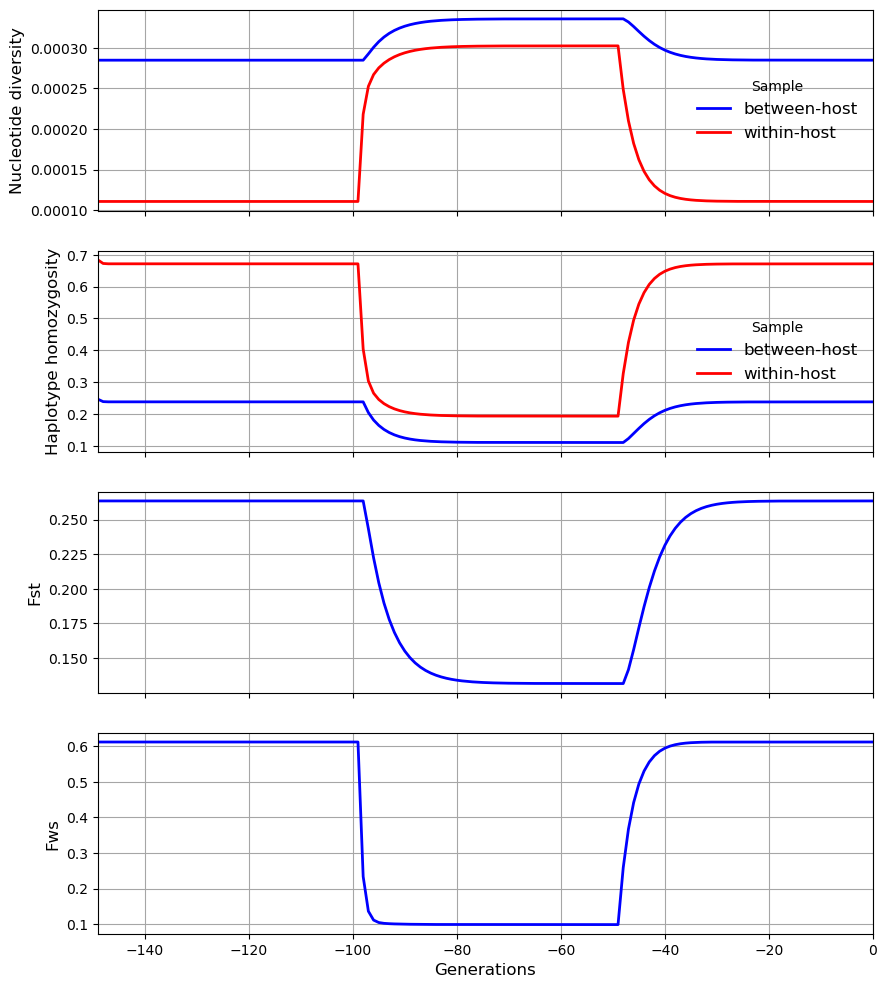
\includegraphics[width=10cm]{230111_scenario_1_3.png}
\caption{\textbf{Increase in the crossing rate of transmission chains.}  In our first scenario $\chi$ transiently increases from 0 to 1 at 100 to 50 generations before the present.  Nucleotide diversity rises, haplotype homozygosity falls
\href{https://github.com/d-kwiat/gtg/blob/main/scenario_1.ipynb}{View code}
}
\label{fig:scenario_1_3}
\end{figure}

In the second scenario, the rate of migration $N_m$ from the metapopulation into the subpopulation transiently increases from 1 to 5 during the period 100 to 50 generations before the present (figure \ref{fig:scenario_1}).   This causes a sharp rise in $\pi_W$, a more modest rise in $\pi_S$ and a sharp fall in $\gamma_W$, $\gamma_S$, $F_{ST}$ and $F_{WS}$.   Thus the effects of an increase in $N_m$ are rather similar to those of an increase in $\chi$.

\begin{figure}[h!]
\centering
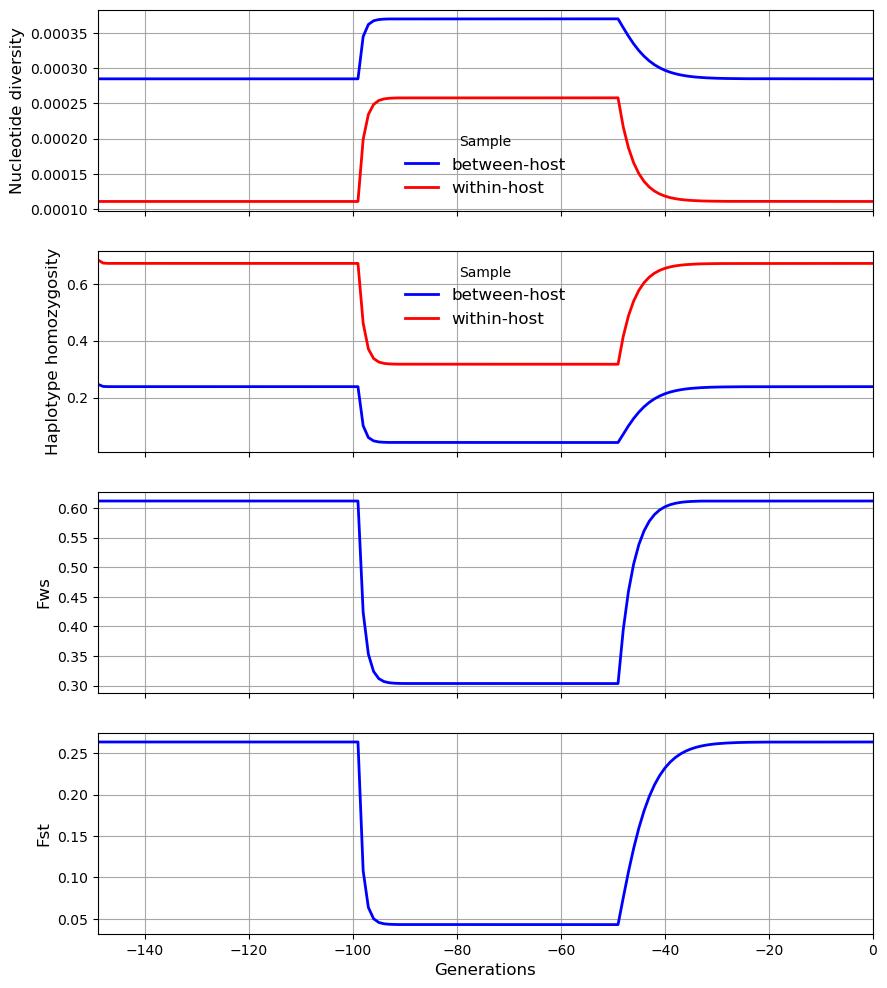
\includegraphics[width=10cm]{230111_scenario_1_4.png}
\caption{\textbf{Increase in the rate of migration from the global metapopulation.}  In this scenario $N_m$ transiently increases from 1 to 5 at 100 to 50 generations before the present.  Nucleotide diversity rises, haplotype homozygosity falls
\href{https://github.com/d-kwiat/gtg/blob/main/scenario_1.ipynb}{View code}
}
\label{fig:scenario_1}
\end{figure}

In the third scenario, the level of $N_h$ in the subpopulation transiently increases from 10 to 30 during the period 100 to 50 generations before the present (figure \ref{fig:scenario_1_2}).   The result is a sharp rise in $F_{WS}$, a modest rise in $F_{ST}$ and $\gamma_W$, a modest fall in $\pi_W$, and small reduction in $\pi_S$.  These results appear paradoxical because we might expect an increase in $N_h$ to cause $\pi_S$ to rise whereas it falls slightly.  The paradox can be explained by recalling that $N_m = m N_h$.  Although $N_m$ is constant, the rise in $N_h$ causes $m$ to decline, and this reduction in the proportion of hosts that have migrated from the metapopulation counterbalances the local increase in effective number of hosts, causing $\pi_S$ to remain almost unchanged.

\begin{figure}[h!]
\centering
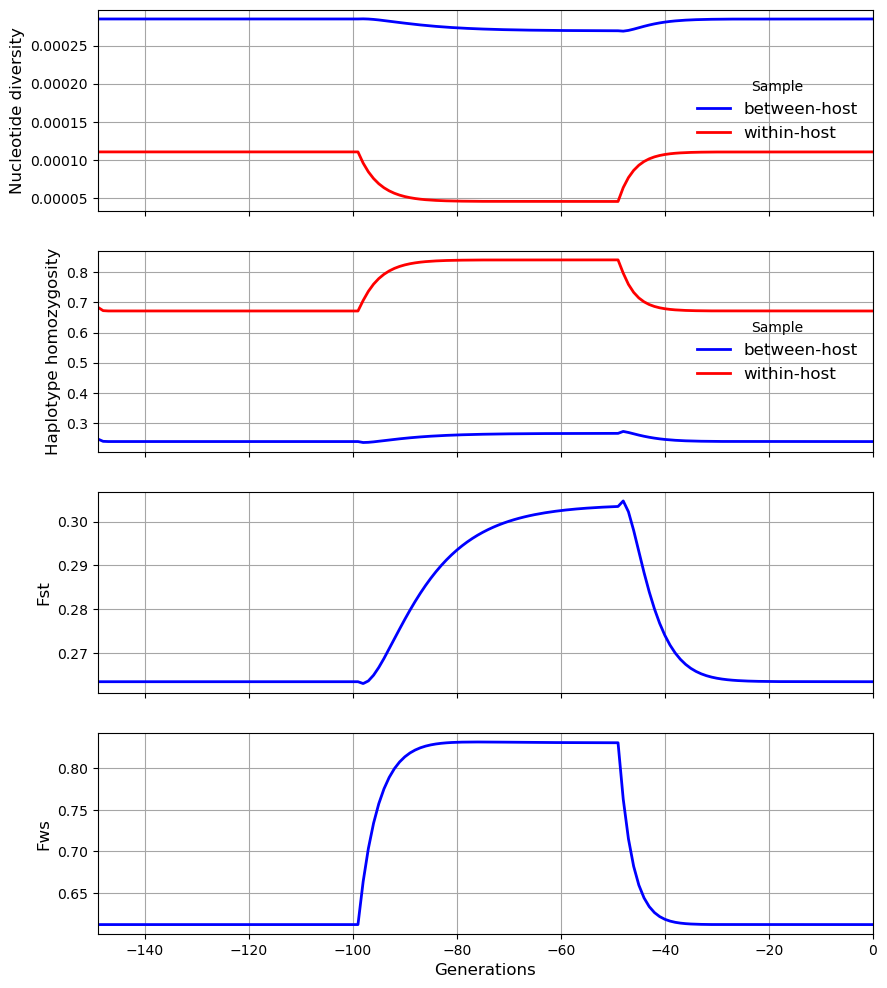
\includegraphics[width=10cm]{230111_scenario_1_2.png}
\caption{\textbf{Increase in the effective number of hosts.}  In this scenario $N_h$ transiently increases from 10 to 30 at 100 to 50 generations before the present.   Paradoxically, nucleotide diversity falls, haplotype homozygosity rises.
\href{https://github.com/d-kwiat/gtg/blob/main/scenario_1.ipynb}{View code}
}
\label{fig:scenario_1_2}
\end{figure}

\end{document}